% !TEX encoding = UTF-8
\documentclass[UTF8]{ctexart}

\usepackage[utf8]{inputenc}
\usepackage{graphicx}
\usepackage{geometry}
\geometry{a4paper}
\geometry{left=2.5cm,right=2.5cm,top=2.8cm,bottom=1.3cm}

\usepackage{booktabs}
\usepackage{array}
\usepackage{paralist}
\usepackage{verbatim}
\usepackage{subfig}
\usepackage{amsmath}
\usepackage{mathtools}
\usepackage{listings}
\usepackage[table]{xcolor}
\usepackage{lastpage}
\usepackage{url}

% Using hyperref for improved ref character
\usepackage[colorlinks,linkcolor=black,anchorcolor=black,
citecolor=black,CJKbookmarks=True]{hyperref}

% For picture drawing
\usepackage[all]{xy}

% For code inserting. Set features.
\lstset{
alsolanguage=matlab,
tabsize=4,
keepspaces=true,
numbers=left,
numberstyle=\tiny,
keywordstyle=\color{blue!70} \bfseries,
commentstyle=\color{red!50!green!50!blue!50},
frame=shadowbox,
breaklines,
showspaces=false,
showstringspaces=false,
showtabs=false,
rulesepcolor=\color{red!20!green!20!blue!20},
extendedchars=false,
escapeinside=``
}

% Set the font of page header
\usepackage{fancyhdr}
\pagestyle{fancy}
\lhead{Step-and-Turn 游戏界面设计与 AI 实现}
\chead{}
\rhead{Page \thepage/\pageref{LastPage}}
\cfoot{}
\rfoot{}
\lfoot{}

\usepackage{sectsty}

\usepackage[nottoc]{tocbibind}
\usepackage[titles,subfigure]{tocloft}
\renewcommand{\cftsecfont}{\rmfamily\mdseries\upshape}
\renewcommand{\cftsecpagefont}{\rmfamily\mdseries\upshape}

% Set number of ref to be relevent to section number
\renewcommand{\theequation}{\arabic{section}.\arabic{equation}}
\renewcommand{\thefigure}{\arabic{section}-\arabic{figure}}
\renewcommand{\thetable}{\arabic{section}-\arabic{table}}
\makeatletter
\@addtoreset{equation}{section}
\@addtoreset{figure}{section}
\@addtoreset{table}{section}
\makeatother

% Set the font of the reference
\bibliographystyle{unsrt}

% Define user\rq{}s color
\usepackage{colortbl}
\definecolor{lightgray}{gray}{.9}
\definecolor{thickgray}{gray}{.6}

\usepackage{multirow}

% 首行缩进
\usepackage{indentfirst}

% Set section numbering
\CTEXsetup[number={}]{part}
\renewcommand{\thepart}{}
\usepackage{titlesec}
\titleformat{\part}[block]{\color{blue}\huge\bfseries\filcenter}{}{1em}{}

%\usepackage{ulem}
%\usepackage{indentfirst}
%\setlength\textwidth{300.0pt}
%

% 重定义字体命令
\newcommand{\song}{\CJKfamily{song}}    % 宋体   (Windows自带simsun.ttf)
\newcommand{\fs}{\CJKfamily{fs}}        % 仿宋体 (华天字库htfs.ttf)
\newcommand{\kai}{\CJKfamily{kai}}      % 楷体   (华天字库htkai.ttf)
\newcommand{\hei}{\CJKfamily{hei}}      % 黑体   (Windows自带simhei.ttf)
\newcommand{\li}{\CJKfamily{li}}        % 隶书   (Windows自带simli.ttf)
\newcommand{\you}{\CJKfamily{you}}      % 幼圆体 (Windows自带simyou.ttf)
%%%  以上六种字体均为标准 GBK 字体, 包括 GBK 繁体字和一些不常用字, 推荐!!!

\newcommand{\xs}{\CJKfamily{xs}}
\newcommand{\shu}{\CJKfamily{shu}}      % 舒体   (方正字库fzstk.ttf)
%  \newcommand{\yourcommand}[参数个数]{内容}   [参数个数]这个是可选的。
%  例如  \newcommand{\you}{\CJKfamily{you}}  用\you 来代替 \CJKfamily{you} ,少输入很多字哦。
%字号设置
\newcommand{\chuhao}{\fontsize{42pt}{\baselineskip}\selectfont}
\newcommand{\xiaochuhao}{\fontsize{36pt}{\baselineskip}\selectfont}
\newcommand{\yihao}{\fontsize{28pt}{\baselineskip}\selectfont}
\newcommand{\xiaoyihao}{\fontsize{24pt}{\baselineskip}\selectfont}
\newcommand{\erhao}{\fontsize{21pt}{\baselineskip}\selectfont}
\newcommand{\xiaoerhao}{\fontsize{18pt}{\baselineskip}\selectfont}
\newcommand{\sanhao}{\fontsize{15.75pt}{\baselineskip}\selectfont}
\newcommand{\sihao}{\fontsize{14pt}{\baselineskip}\selectfont}
\newcommand{\xiaosihao}{\fontsize{12pt}{\baselineskip}\selectfont}
\newcommand{\wuhao}{\fontsize{10.5pt}{\baselineskip}\selectfont}
\newcommand{\xiaowuhao}{\fontsize{9pt}{\baselineskip}\selectfont}
\newcommand{\liuhao}{\fontsize{7.875pt}{\baselineskip}\selectfont}
\newcommand{\qihao}{\fontsize{5.25pt}{\baselineskip}\selectfont}
% \baselineskip | distance from bottom of one line of a paragraph to bottom of the next line.  基本行距
%  只有使用\selectfont命令之后,\fontzize{}{}的设置才能生效
%  可以用数字表示{11pt}:单倍行距

\begin{document}
%%%%%%%%%%%%%%%%%%%%%%%%%%%%封面与目录%%%%%%%%%%%%%%%%%%%%%%%%%%%%%%
\begin{titlepage}
\begin{center}
% Upper part of the page

\includegraphics[width=0.25\textwidth]{pic/logo.jpg}\\[1cm]
\textsc{\LARGE Department of Automation}\\[1.5cm]
\fs{\Large 人工智能搜索大作业报告}\\[0.5cm]
% Title
\hrulefill
\\[0.8cm]{\centering \huge \hei Step-and-Turn 游戏界面设计与 AI 实现}\\[0.4cm]
\hrulefill
\\[4cm]

% Author and supervisor
\begin{tabbing}       %tabbing  列表

 \hspace*{5cm} \= \hspace{2.6cm} \= \kill
 % \=     in tabbing environment, sets a tab stop
 % \kill  in a\tabbing environment, deletes previous line so tabs can be set without outputting text.
 % \>     in tabbing environment is a forward tab.

\>{\fs\sihao\textbf {班\hspace{1cm}级 \ \ :}}\>  {\centering\fs\sihao\textbf{~~~~~~~~~自~~3~2}} \\
\\
\>{\fs\sihao\textbf {姓\hspace{1cm}名 \ \ :}}\>  {\centering\fs\sihao\textbf{~~~~~~~~陈~昊~楠}}\\
\\
\>{\fs\sihao\textbf {学\hspace{1cm}号 \ \ :}}\>  {\centering\fs\sihao\textbf{~~~~~~2013011449}}\\
\\
\>{\fs\sihao\textbf {授课教师 \ \ :}}\>  {\centering\fs\sihao\textbf{~~~~~~~~张~长~水}} \\

\end{tabbing}
\vfill
{\large \today}
\end{center}
\end{titlepage}

\tableofcontents
\clearpage

%%%%%%%%%%%%%%%%%%%%%%%%%%正文部分%%%%%%%%%%%%%%%%%%%%%%%%%%%%%%%%%%

\section{声明}
\begin{itemize}
\item 本作业使用评分模板B;
\item 程序使用{\ttfamily Python}开发,游戏界面使用{\ttfamily pygame}框架;
\item 运行环境为 {\ttfamily Windows10}操作系统。
\end{itemize}

\section{Step-and-turn游戏规则}
该游戏是作者自创的。规则为:
\begin{itemize}
	\item 两名游戏者轮流行动;
	\item 棋盘上有棋子和障碍物,游戏者每人控制一些棋子;
	\item 每个棋子有四个方向,棋子可能的行动为沿当前方向向前一步(step)和通过左转、右转变换方向(turn);
	\item 轮到某位游戏者时,游戏者先选择一枚棋子进行移动,后选择一枚棋子进行旋转,所选棋子可以相同,也可以不同;
	\item 移动后不得与障碍物、本方其他棋子和对方棋子重叠;
	\item 率先无法移动的游戏者判为失败。
\end{itemize}

注意,规则中并没有要求双方棋子数相同,也没有规定具体的棋盘模式。在程序实现时,将游戏定位为闯关式,双方一般是不平衡的。

\section{UI设计}
\paragraph{开始界面}
游戏开始界面如图\ref{fig:startscreen}所示。其中艺术字使用{\ttfamily Adobe PhotoShop}绘制,并给出了游戏用法的提示:
\begin{figure}[htbp]
\centering
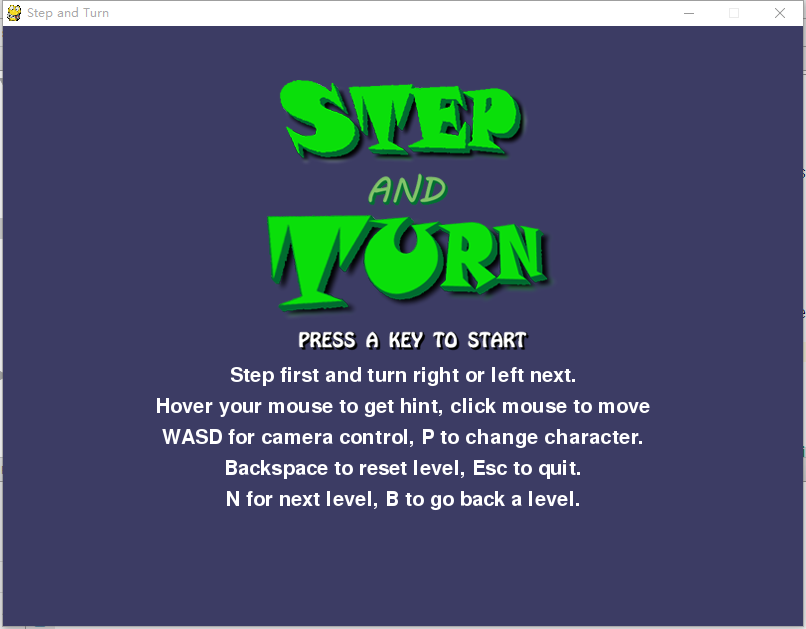
\includegraphics[width=11cm]{pic/startscreen.png}
\caption{Step-and-Turn开始界面}
\label{fig:startscreen}
\end{figure}

\paragraph{游戏界面}
按任意键将从开始界面进入游戏主界面,如图\ref{fig:ui}。程序将从已有的地图文件中读入地图信息,并装饰地图。界面右下角提示了当前关卡,总关卡数和当前行动的玩家。
\begin{figure}[htbp]
\centering
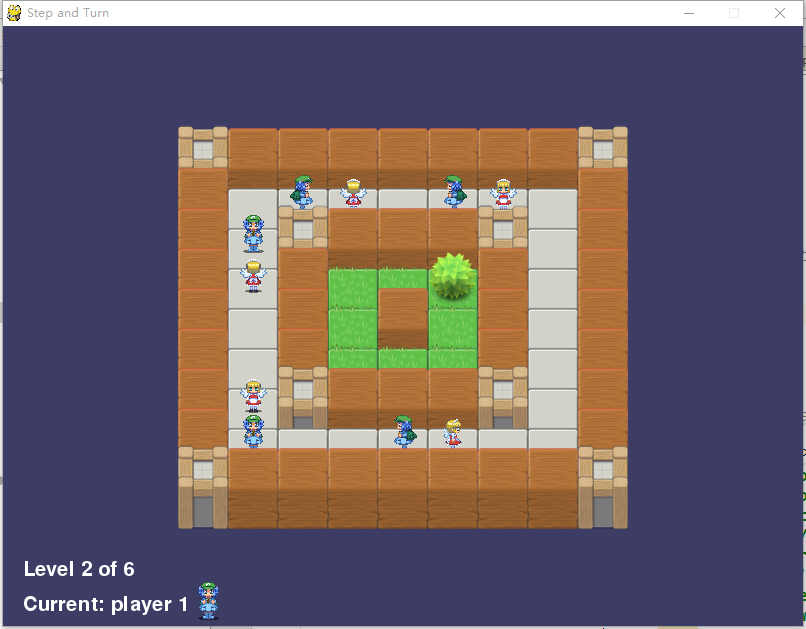
\includegraphics[width=11cm]{pic/ui.png}
\caption{Step-and-Turn主界面}
\label{fig:ui}
\end{figure}

操作方法已在开始界面说明,即:
\begin{itemize}
	\item 将鼠标悬停在人物上可以获得提示,如图\ref{fig:stephint}和图\ref{fig:turnhint},点击鼠标可以进行移动。当处于前进状态时,直接点击人物或提示位置;处于旋转状态时,点击人物两边的方块作为目标朝向。
	\item 当地图较大无法看清全貌时,可以使用{\ttfamily WASD}键移动画面。
	\item {\ttfamily P}键切换当前玩家的人物。游戏在每次启动都会随机选取人物,且切换之后在所有关卡都生效。
	\item {\ttfamily Esc}键退出,空格键重置当前关,{\ttfamily N}进入下一关,{\ttfamily B}退回上一关。
\end{itemize}

\begin{figure}[htbp]
\begin{minipage}[t]{0.5\linewidth}
\centering
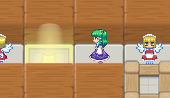
\includegraphics[width=3in]{pic/stephint.png}
\caption{前进提示}
\label{fig:stephint}
\end{minipage}
\begin{minipage}[t]{0.5\linewidth}
\centering
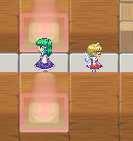
\includegraphics[width=2in]{pic/turnhint.png}
\caption{旋转提示}
\label{fig:turnhint}
\end{minipage}
\end{figure}

\paragraph{地图文件说明}
可以自行撰写地图文件。默认地图文件为根目录下的{\ttfamily stepturnLevel.txt}文件。撰写规则为:
\begin{itemize}
	\item 分号所在行为注释;
	\item 地图之后须有至少一个空行;
	\item \# 号为障碍物;
	\item 玩家一的上、右、下、左四个方向分别为(大写){\ttfamily W, A, S, D},玩家二为{\ttfamily I, J, K, L}。
\end{itemize}

\paragraph{地图装饰方案}
由文件读入地图后,游戏程序将对地图进行装饰处理。方案如下:
\begin{itemize}
	\item 障碍物处在边上,使用土墙;
	\item 障碍物处在边上,使用栅栏;
	\item 以所有人物所在位置为种子点使用 Flood Fill 算法确定内部位置,使用石砖;
	\item 外部空地使用草坪,并随机装饰树、丛、石头等物品。
\end{itemize}

\paragraph{游戏数学逻辑}
游戏中

\end{document}
